\documentclass[xcolor=pdftex,dvipsnames,table]{beamer}
%\usepackage{subfigure}
\usepackage{amsbsy}
\usepackage{tikz}
\usetikzlibrary{arrows}
\usepackage{amsmath,graphicx,dsfont,color}
\usepackage{amsfonts}
\usepackage{amssymb}
\usepackage{array}

\usepackage{subfig}

% makes the subfig package work
\makeatletter
\let\@@magyar@captionfix\relax
\makeatother

% subfigure counter resets every frame
\makeatletter
\@addtoreset{subfigure}{framenumber}
\makeatother

% First author and year
\bibliographystyle{apalike}

% This sets the list items of the bibliography to the same symbol used for citation.
\setbeamertemplate{bibliography item}{\insertbiblabel}

% This avoids extralines for different entries
\setbeamertemplate{bibliography entry title}{}
\setbeamertemplate{bibliography entry location}{}
\setbeamertemplate{bibliography entry note}{}

\DeclareMathOperator*{\argmin}{arg\,min}
\DeclareMathOperator*{\argmax}{arg\,max}
%Definitiona

\newcommand{\x}{\mathbf{x}}
\newcommand{\X}{\mathbf{X}}
\newcommand{\W}{\mathbf{W}} %Weight
\newcommand{\bais}{\mathbf{b}}%Bais
\newcommand{\act}{\texttt{g}}%Activation
\newcommand{\loss}{L}
\newcommand{\pdata}{\hat{p}_{\texttt{data}}}
\newcommand{\nsize}{N}
\newcommand{\nfeatures}{P}
\newcommand{\param}{\boldsymbol{\theta}}
\newcommand{\featmap}{\boldsymbol{\phi}}
\newcommand{\EV}{\mathbb{E}}









\title{Deep Learning for Image Analysis - \\ 
	   Lecture 1: An introduction to Machine Learning}
\author{Thomas Walter, PhD}
\date{Centre for Computational Biology (CBIO) \\
	  MINES Paris-Tech, PSL Research University \\
	  Institut Curie, PSL Research University \\
	  INSERM U900}


%To include LOGO?
%\logo{\includegraphics[width=.1\columnwidth]{MinesLogo}}
\useinnertheme{rounded}
\usecolortheme{rose}

\usepackage{xcolor}
\definecolor{lightblue}{RGB}{0,200,255}


\setbeamertemplate{footline}[frame number]{}
\setbeamertemplate{navigation symbols}{}
\setbeamertemplate{section in toc}[square]
\setbeamertemplate{items}[square]


\begin{document}

\begin{frame}
\titlepage
\end{frame}

\begin{frame}{Overview}
\tableofcontents
\end{frame}

%%%%%%%%%%%%%%%%%%%%%%%%%%%%%%%%%%%%%%%%%%%%%%%%%%%%%%%%%%%%%%%%%%%%%%%%%
%%%%%%%%%%%%%%%%%%%%%%%%%%%%%%%%%%%%%%%%%%%%%%%%%%%%%%%%%%%%%%%%%%%%%%%%%
\section{Introduction: Artificial Intelligence and Machine Learning}
\frame{\frametitle{Overview}\tableofcontents[currentsection]}

\begin{frame}{Definition of Artificial Intelligence and Machine Learning}
%\begin{definition}
%	Artificial intelligence (AI) is intelligence demonstrated by machines, in contrast to the natural intelligence displayed by humans and other animals.
%\end{definition}
\begin{itemize}
	\item The definition of the term \textbf{intelligence} is highly controversial. Usually, one understands by intelligence the capacity of an individual to reason logically, to understand complexity, to learn more or less abstract concepts, to plan and to solve problems in varying conditions. 	
	\item \textbf{Artificial intelligence (AI)} is intelligence demonstrated by machines, in contrast to the natural intelligence displayed by humans and other animals. 
	\item AI effect: \emph{"AI is whatever hasn't been done yet"}.
	\item In 1956, AI became a field of research. AI can be broken down into many subfields: knowledge representation, planning, natural language processing, object manipulation (robotics), machine learning, $\ldots$
	\item \textbf{Machine Learning} is concerned with the technology that enables computer programs to improve their performance at a certain task by experience.
\end{itemize}
\end{frame}

\begin{frame}{A short history of artificial intelligence}
\begin{itemize}
	\item The dream to create machines that can think and act has been present in literature and mythology since antiquity (e.g. the myth of \emph{"Talos"} or \emph{"Rossum's Universal Robots"} by Karel \v{C}apek, 1920).
	\item AI as a scientific discipline took its beginning with the publication of Alan Turing in 1950 (Turing test). The question \emph{"Can machines think?"} was asked scientifically.
	\item Other theoretical bases were developed by Wiener (cybernetics) and Shannon (information theory). 
	\item The term \emph{"artificial intelligence"} was cornered in 1956, in the famous Dartmouth conference, where AI has been established as a field.
\end{itemize}
\end{frame}

\begin{frame}{A short history of machine learning}
\begin{itemize}
	\item The theoretical foundations go back to the early 19th century (e.g. Bayesian theory and Least Squares). 
	\item Even before machines came into play, there was a lot of interest in finding methods to derive rules from data (\emph{data fitting}). These methods are part of what we call Machine Learning today (linear regression, Bayesian theory, Logistic regression, Linear discriminant analysis, Markov chains). 
	\item In 1958, Rosenblatt published his \emph{Perceptron}. 
\end{itemize}
\end{frame}

\begin{frame}{Machine Learning: basic definitions}
\begin{itemize}
	\item Machine Learning aims at predicting some output $y$ from an input (or measurement) $x$:
	\begin{equation}
	y = f(x)
	\end{equation}
	\item In this formulation, Machine Learning aims at finding (learning) $f$ from available data. 
	\item The data that is used to learn $f$ is called \textbf{training set}. 
	\item In this general formulation, there is no particular limitation as to the mathematical nature of $x$ and $y$. In many cases $x$ is a $\nfeatures$-dimensional vector and $y$ a categorical or continuous output variable, but there are other settings, where $x$ and / or $y$ are more complicated objects, such as images or graphs.
\end{itemize}
\end{frame}

\begin{frame}{Different settings in Machine Learning}
	\begin{table}
	\begin{tabular}{|l || c | c | }
		\hline
 		& Supervised & Unsupervised \\
		\hline \hline
		$y$ discrete & Classification & Clustering \\ 
		$y$ continuous & Regression & Dimensionality reduction\\ 
		\hline
	\end{tabular}
	\end{table}
\begin{itemize}
	\item In \textbf{supervised learning}, the training data contains both measurements $x_i$ and the corresponding output variables $y_i$. Together, they build the training set $T$:
	\begin{equation}
	T = \{(x_i, y_i)\}_{i=1, \ldots, \nsize}
	\end{equation}
	\item In \textbf{unsupervised learning}, there are no annotations $y_i$. We aim at inferring \textbf{patterns} from the data (clusters, latent variables). 
\end{itemize}
\end{frame}

\begin{frame}{Training and prediction}
\begin{figure}[htb]
  \centering
  \subfloat[Training a classifier]{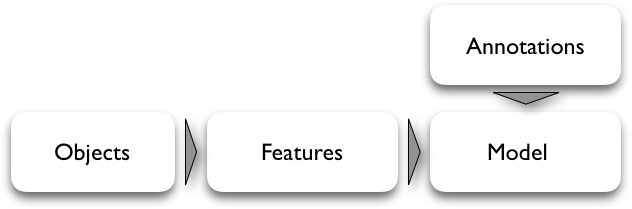
\includegraphics[width=0.6\textwidth]{../graphics/workflow_training.png}}\\  
  \subfloat[Prediction]{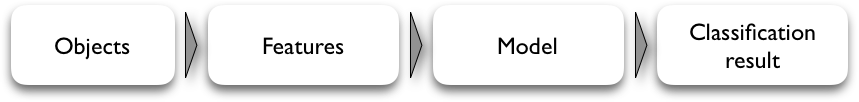
\includegraphics[width=0.8\textwidth]{../graphics/workflow_prediction.png}} 
\end{figure}
\begin{itemize}
\item Training: to learn a model from the training set. Depending on the method, this can take minutes, hours or days.
\item Prediction: to apply the learned classifier to new data. This is usually computationally efficient. 
\end{itemize}
\end{frame}

\begin{frame}{Objects and features}
\begin{itemize}
\item Machine learning typically deals with objects outside the mathematical world (emails, images, genomes, cars, $\ldots$).
\item The first step is therefore to find a suitable representation of the objects. 
\begin{itemize}
\item \textbf{feature engineering}: finding descriptors according to existing domain knowledge
\item \textbf{representation learning}: learning the descriptors together with the classifier
\end{itemize}
\item In many cases the objects can be represented by a $\nfeatures$-dimensional vector of features (or descriptors): $\x \in \mathbb{R}^{\nfeatures}$. 
\item It can be convenient to map a feature vector to a higher dimensional space:
\begin{eqnarray}
\featmap : \mathbb{R}^{\nfeatures} &\rightarrow & \mathbb{R}^Q \\
\x &\rightarrow &\featmap (\x)
\end{eqnarray}
\end{itemize}
\end{frame}

\begin{frame}{Training set and design matrix}
\begin{itemize}
\item In the frequent case that objects can be described by a feature vector $\x \in \mathbb{R}^{\nfeatures}$, we can represent the training set $T = \{(x_i, y_i)\}_{i=1, \ldots, \nsize}$ by a $\nsize \times \nfeatures$ \textbf{design matrix} $\X$ and an output vector $y$.
\item In the design matrix, each row corresponds to one sample, each column corresponds to one feature: 
\begin{table}
\begin{tabular}{|l || c | c | c | c |}
	\hline
		& feature 1 & feature 2 & $\ldots$ & feature $\nfeatures$ \\
	\hline \hline
	Sample 1 & 0.23 & 1.30 & $\ldots$ & 0.01 \\ 
	\hline
	Sample 2 & 0.42 & 1.15 & $\ldots$ & -0.23 \\ 
	\hline
	$\vdots$ & $\vdots$ & $\vdots$ & $\vdots$ & $\vdots$ \\ 
	\hline
	Sample $\nsize$ & 0.31 & 1.53 & $\ldots$ & 0.33 \\ 
	\hline
\end{tabular}
\end{table}
\end{itemize}
\end{frame}


\begin{frame}{Example: classification of flowers}
\begin{figure}
  \centering
  \subfloat[Iris setosa]{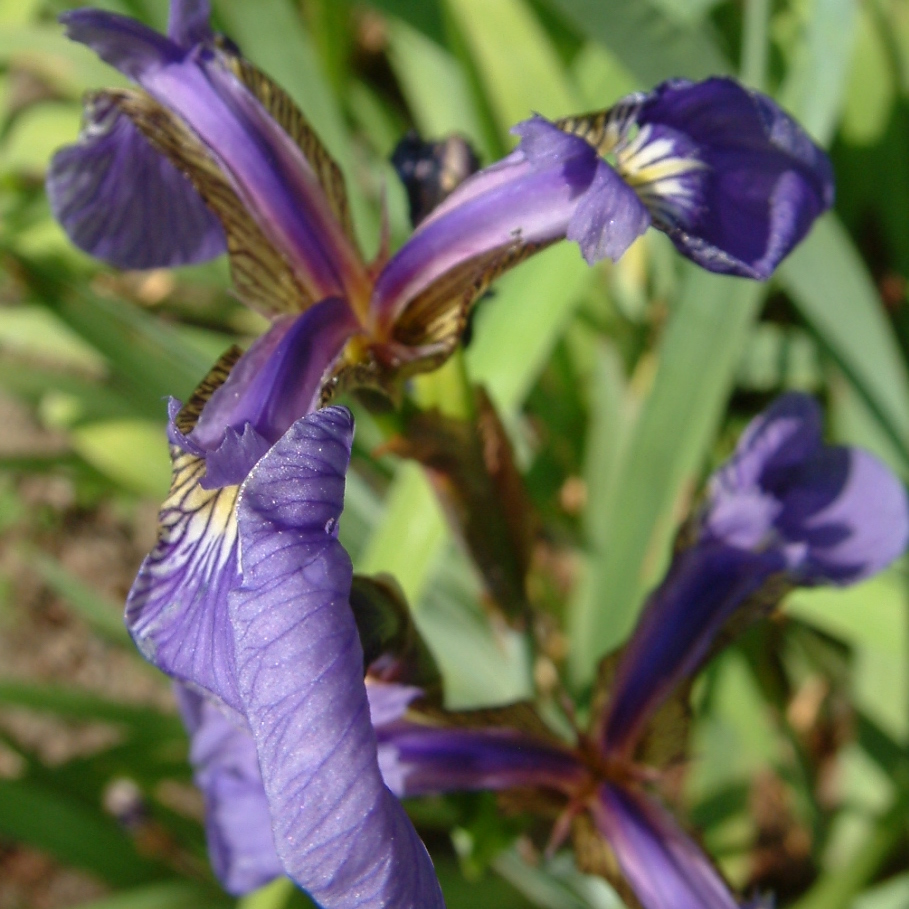
\includegraphics[height=2.4cm]{../graphics/Iris_setosa.jpg}}\qquad    
  \subfloat[Iris versicolor]{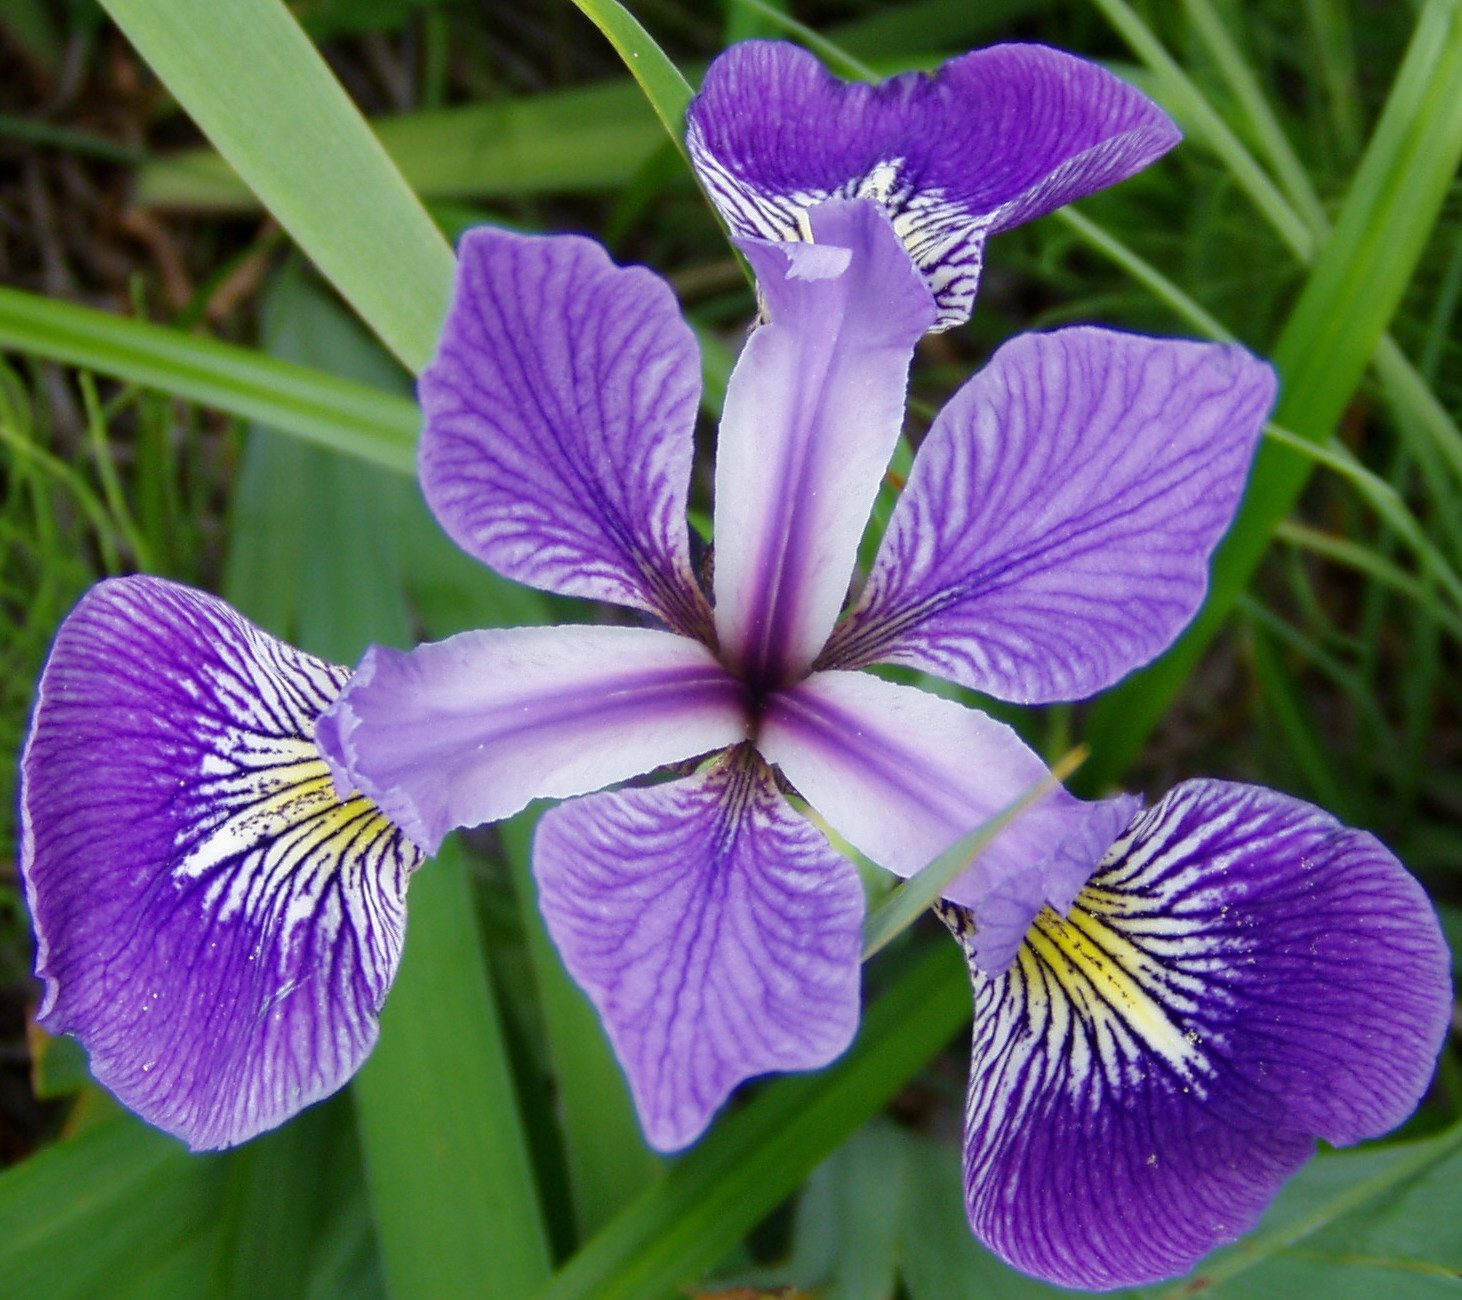
\includegraphics[height=2.4cm]{../graphics/Iris_versicolor.jpg}}\qquad
  \subfloat[Iris virginica]{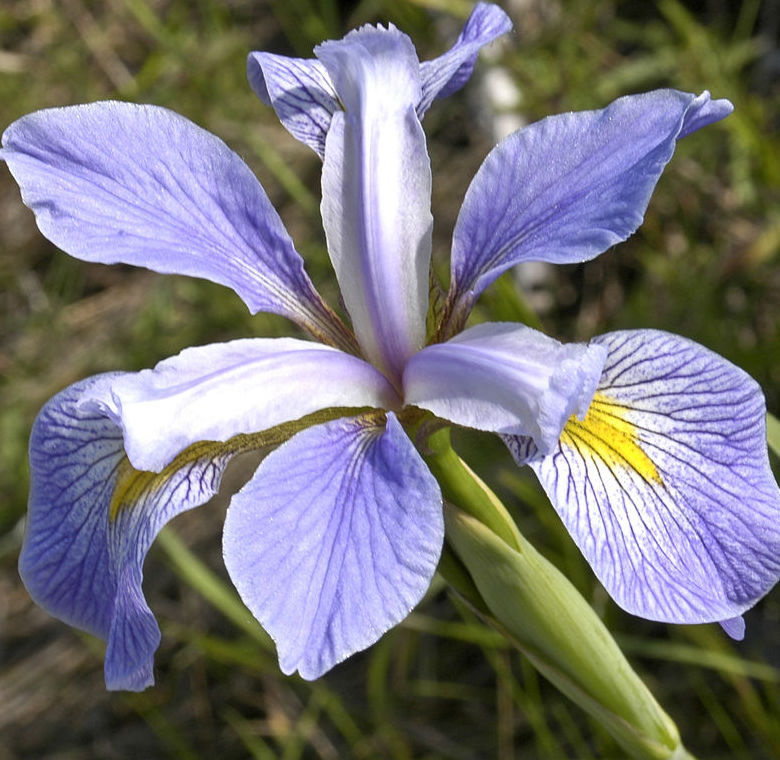
\includegraphics[height=2.4cm]{../graphics/Iris_virginica.jpg}}\qquad
  \label{fig:Iris_data_set}
\end{figure}
\begin{itemize}
	\item One of the oldest data sets in machine learning is the Iris data set, that was collected by the statistician and biologist Ronald Fisher in 1936 \cite{Fisher1936}. 
	\item There are 3 classes (different types of the Iris flower). For each class, there were 50 samples collected. For each sample, 4 characteristics were measured (lengths and widths of different parts of the plants).
	\item The task is thus to learn a rule to predict the type of the flower ($y$) from a 4-dimensional vector $x$ of geometric measurements. 
\end{itemize}
\end{frame}

\begin{frame}{Example: classification of SPAM emails}
\begin{figure}[htb]
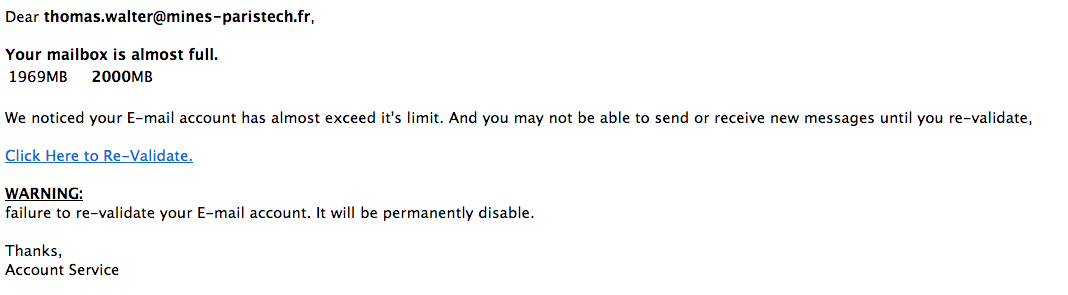
\includegraphics[width=0.9\textwidth]{../graphics/SPAM_mail.png}
\end{figure}
\begin{itemize}
	\item This is a binary classification problem: $y \in \{0,1\}$ (0: junk, 1: normal). 
	\item The features can be constructed in the following way: for each email annotated by the user, the words are listed. An email is described as a vector of frequencies of these words. 
	\item The system learns then a function that assigns to each vector of measured word frequencies the label $y$. 
\end{itemize}
\end{frame}

\begin{frame}{Example: classification of drugs}
\begin{figure}[htb]
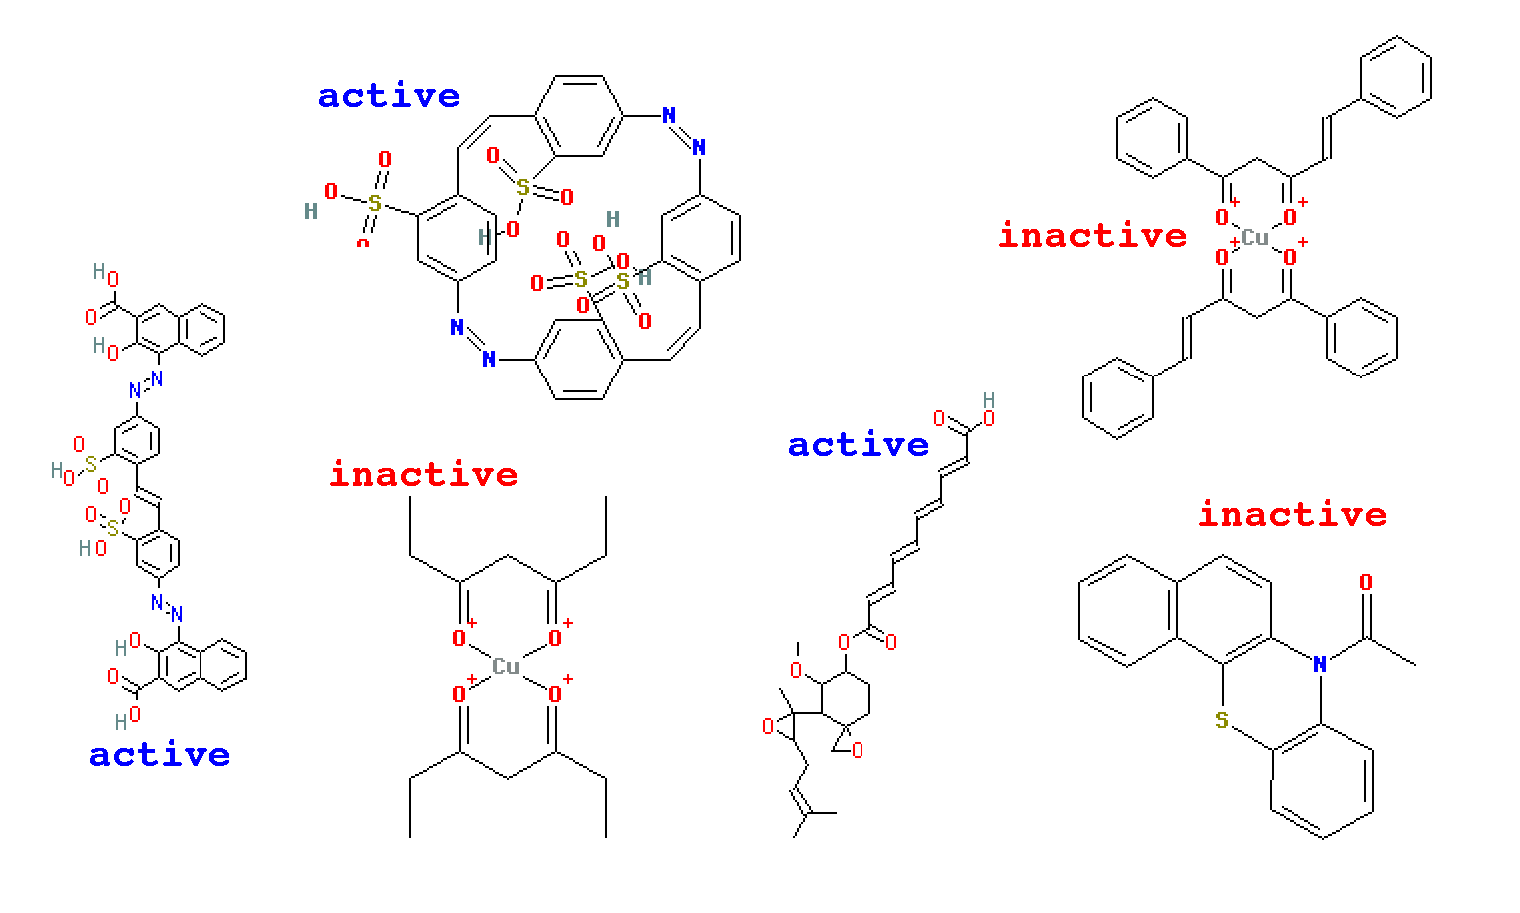
\includegraphics[width=0.7\textwidth]{../graphics/ml_example_drugs.pdf}
\end{figure}
\begin{itemize}
	\item Here, we want to classify molecules with respect to their efficiency against a disease (binary classification: a drug is efficient or not). 
	\item An important question here is how to encode a molecule. One option is to define chemoinformatic features and obtain a vectorial representation of the molecule $\x \in \mathbb{R}^{\nfeatures}$. 
\end{itemize}
\end{frame}


%%%%%%%%%%%%%%%%%%%%%%%%%%%%%%%%%%%%%%%%%%%%%%%%%%%%%%%%%%%%%%%%%%%%%%%%%
%%%%%%%%%%%%%%%%%%%%%%%%%%%%%%%%%%%%%%%%%%%%%%%%%%%%%%%%%%%%%%%%%%%%%%%%%
\section{Design Principles of Machine Learning algorithms}
\frame{\frametitle{Overview}\tableofcontents[currentsection]}

\begin{frame}{A simple example: polynomial curve fitting\footnote{Example adapted from \cite{Bishop2006}}}
\begin{figure}[htb]
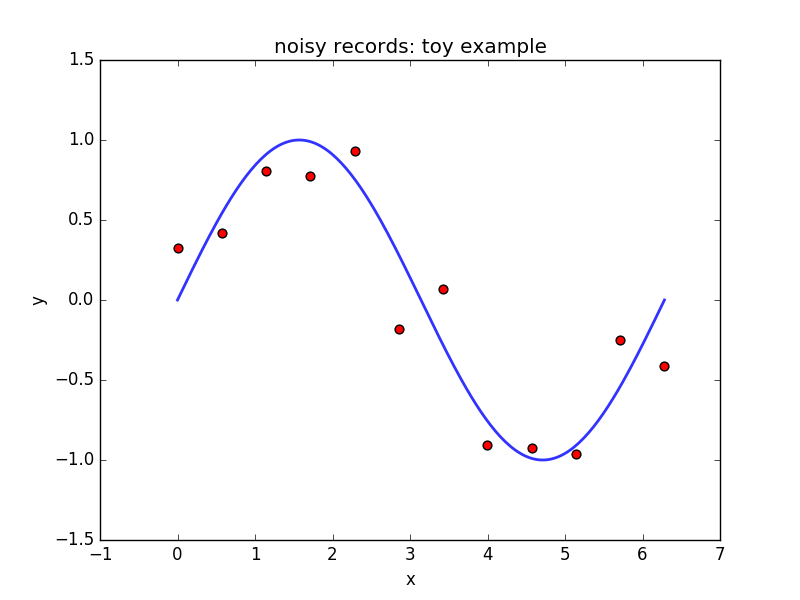
\includegraphics[width=0.6\textwidth]{../graphics/sample_from_sin.png}
\end{figure}
\begin{itemize}
	\item From a set of measured points $(x_i, y_i)$ (red), we would like to build a model to predict the value $y$ for any given $x$. 
	\item The true function is $g(x)=\sin (x)$ (displayed in blue).
	\item The measurements $y_i$ are noisy outputs of that function, i.e. 
	\begin{equation}
	y_i = \sin (x_i) + \epsilon \; , \;\;\; \;\;\; \epsilon \sim \mathcal{N}(0,0.2)
	\end{equation}
\end{itemize}
\end{frame}

\begin{frame}{A simple example: polynomial curve fitting}
\begin{itemize}
	\item We use the following polynomial model:
	\begin{eqnarray}
	f(x) &=& a_0 + a_1 x + a_2 x^2 + \ldots + a_m x^m \nonumber \\
	&=& \param^T \featmap (x)
	\end{eqnarray}
	\item Parameter vector: $\param = (a_0, a_1, \ldots, a_m)^T$
	\item Here, the initial measurement $x$ is a scalar. In our model, we map $x$ to a higher dimensional space: 
	\begin{eqnarray}
		\featmap : \mathbb{R}^{\nfeatures} &\rightarrow & \mathbb{R}^Q \nonumber \\
		x &\rightarrow & \featmap (x) = (1, x, x^2, \ldots, x^m)^T
	\end{eqnarray}
	\item The model is linear in the parameters $\theta$ and linear in $\featmap$, but for $m>1$, the model is not linear in $x$. 
\end{itemize}
\end{frame}

\begin{frame}{A simple example: polynomial curve fitting}
\begin{itemize}
	\item One classical approach is to minimize the least squared error between measured and predicted values:
	\begin{eqnarray}
		\min_{\param} \loss(\param) &=& \min_{\param} \sum_{i=1}^N (y_i - f(x_i))^2 \nonumber \\
		&=& \min_{\param} \sum_{i=1}^N (y_i - \param^T \featmap (x_i))^2 
	\end{eqnarray}
	\item This can be achieved by setting the gradient with respect to $\param$ to zero:
	\begin{equation}
		\nabla_{\param} \loss = (\frac{\partial \loss}{\partial a_0}, \frac{\partial \loss}{\partial a_1}, \ldots, \frac{\partial \loss}{\partial a_m} )^T = 0
	\end{equation}
	\item Unlike for most optimization problems in this course, this leads to an analytical solution for $\param$. This is known as \textbf{linear regression}. For more details, we refer to \cite{Hastie2009}.
\end{itemize}
\end{frame}

\begin{frame}{Overfitting and underfitting}
\begin{figure}[htb]
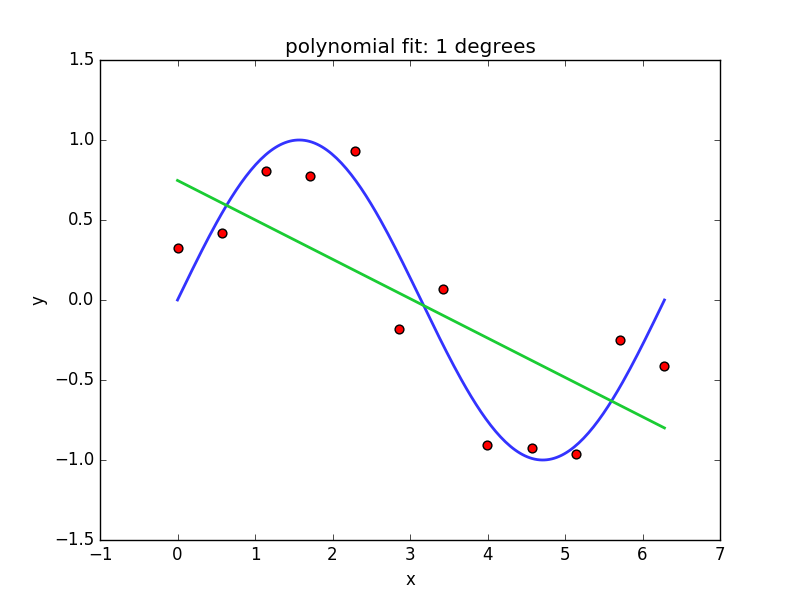
\includegraphics[width=0.6\textwidth]{../graphics/polyfit_degree_1.png}
\end{figure}
For $m=1$, the model is linear in its inputs. The solution is not capable of modeling the measured data points; we get a poor approximation of the original function. The family of functions we have used was not complex enough to model the true data distribution. We also speak of \textbf{underfitting}.
\end{frame}

\begin{frame}{Overfitting and underfitting}
\begin{figure}[htb]
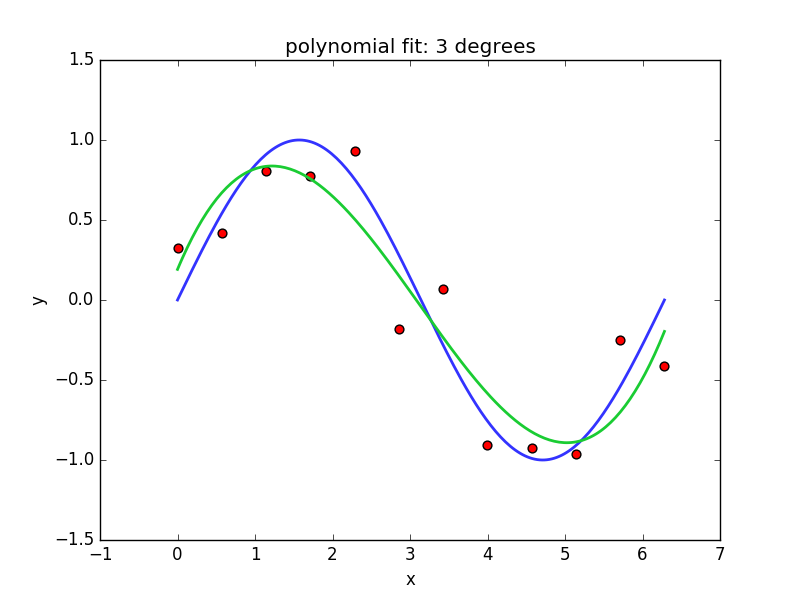
\includegraphics[width=0.6\textwidth]{../graphics/polyfit_degree_3.png}
\end{figure}
For $m=3$, we obtain a solution that seems to be quite right: it is sufficiently complex to model the true data distribution, but not too complex to model the small variations which are due to noise.
\end{frame}

\begin{frame}{Overfitting and underfitting}
\begin{figure}[htb]
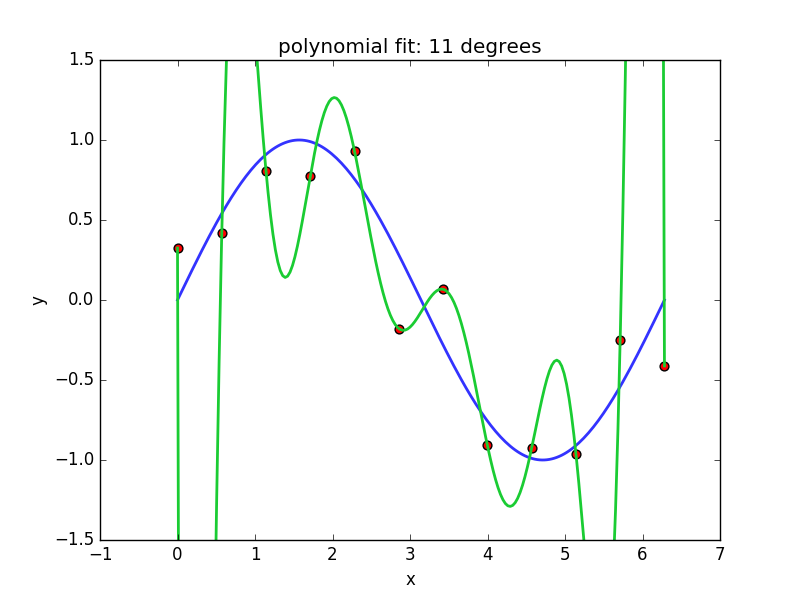
\includegraphics[width=0.6\textwidth]{../graphics/polyfit_degree_11.png}
\end{figure}
For $m=11$, we obtain a solution that has zero error (the function passes through every point of the training set). But the coefficients with large absolute values that cancel each other precisely on the training points lead to a highly unstable function. We speak of \textbf{overfitting} and \textbf{poor generalization}.
\end{frame}

\begin{frame}{Overfitting and underfitting}
\begin{figure}[htb]
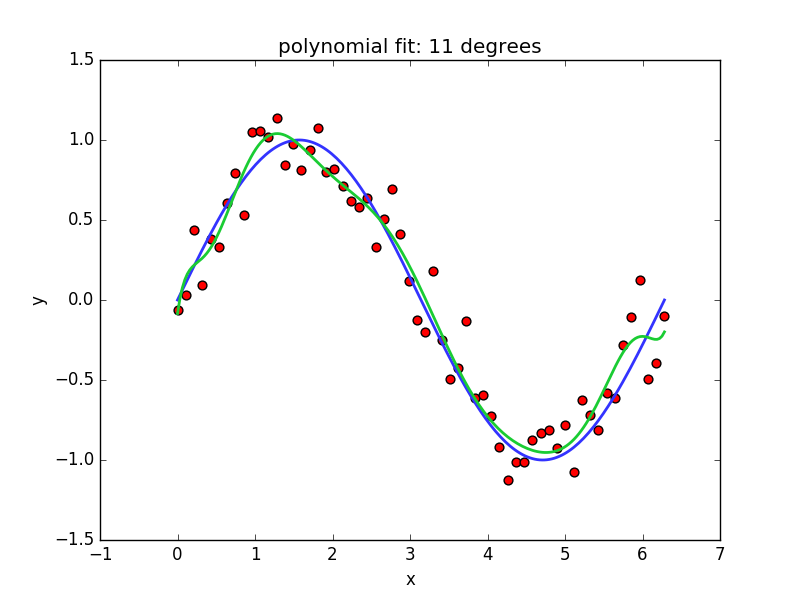
\includegraphics[width=0.6\textwidth]{../graphics/polyfit_degree_11_N60.png}
\end{figure}
One way of reducing overfitting is to increase the number of samples. Even if the function is complex, it cannot be “too wild”, as it has to find a compromise between many training samples. This however implies the annotation (or measurement) of more samples. 
\end{frame}

\begin{frame}{Overfitting and underfitting}
\begin{figure}[htb]
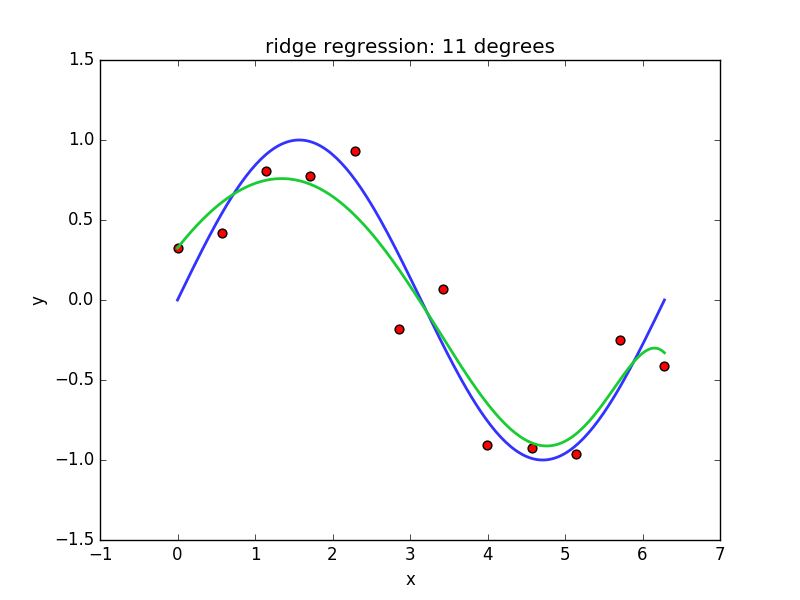
\includegraphics[width=0.6\textwidth]{../graphics/ridge_regression_11_10.png}
\end{figure}
Another way of preventing overfitting without increasing the number of samples, is to add a penalization term in the optimization procedure. This is also known as \textbf{regularization}:
\begin{equation}
	\loss = \sum_{i=1}^N (y_i - \param^T \featmap (x_i))^2 + \lambda \| \param \|^2
\end{equation}
\end{frame}

\begin{frame}{Generalization: training and test error}
\begin{figure}[htb]
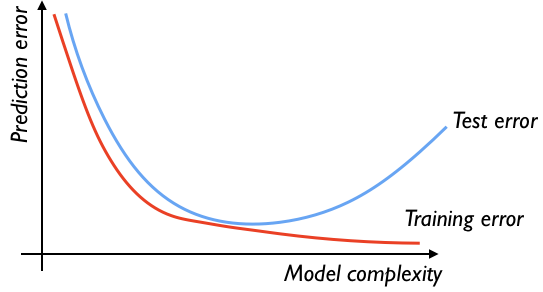
\includegraphics[width=0.6\textwidth]{../graphics/Training_and_test_error.png}
\end{figure}
\begin{itemize}
\item Supervised Learning aims at finding a function $f$ that predicts an output value $y$ from a measurement $x$ for unseen data, i.e. for data that has not been used to find $f$. 
\item Machine Learning is much concerned with avoiding $f$ to \textbf{memorize} the training set, i.e. to perform well on a training set but poorly a test set. 
\item An important paradigm is that we must never evaluate the performance of our machine learning method on the data that has been used to train it.
\end{itemize}
\end{frame}

\begin{frame}{Generalization: strategies}
\begin{itemize}
\item Many ML algorithms can be written as an optimization problem:
\begin{equation}
\param ^{\ast} = \argmin_{\param} \loss (\param) + \mathcal{R}(\param)
\end{equation}
Minimizing the loss $\loss (\param)$ aims at finding the rule to reproduce the annotations in the training set, minimizing the regularization term $\mathcal{R}(\param)$ aims at avoiding the model to adapt too much to the training data, leading to simpler models. We have seen the $L_2$ norm, but there are many other options for $\mathcal{R}$. 
\item Other regularization strategies include:
\begin{itemize}
\item Model averaging (ensemble methods)
\item Artificial or actual increase of training data
\item Adversarial training
\end{itemize}
\end{itemize}
\end{frame}

%%%%%%%%%%%%%%%%%%%%%%%%%%%%%%%%%%%%%%%%%%%%%%%%%%%%%%%%%%%%%%%%%%%%%%%%%
%%%%%%%%%%%%%%%%%%%%%%%%%%%%%%%%%%%%%%%%%%%%%%%%%%%%%%%%%%%%%%%%%%%%%%%%%
\section{Supervised Learning: Example algorithms}

% \begin{frame}{Example: classification of cells}
% \begin{figure}[htb]
% 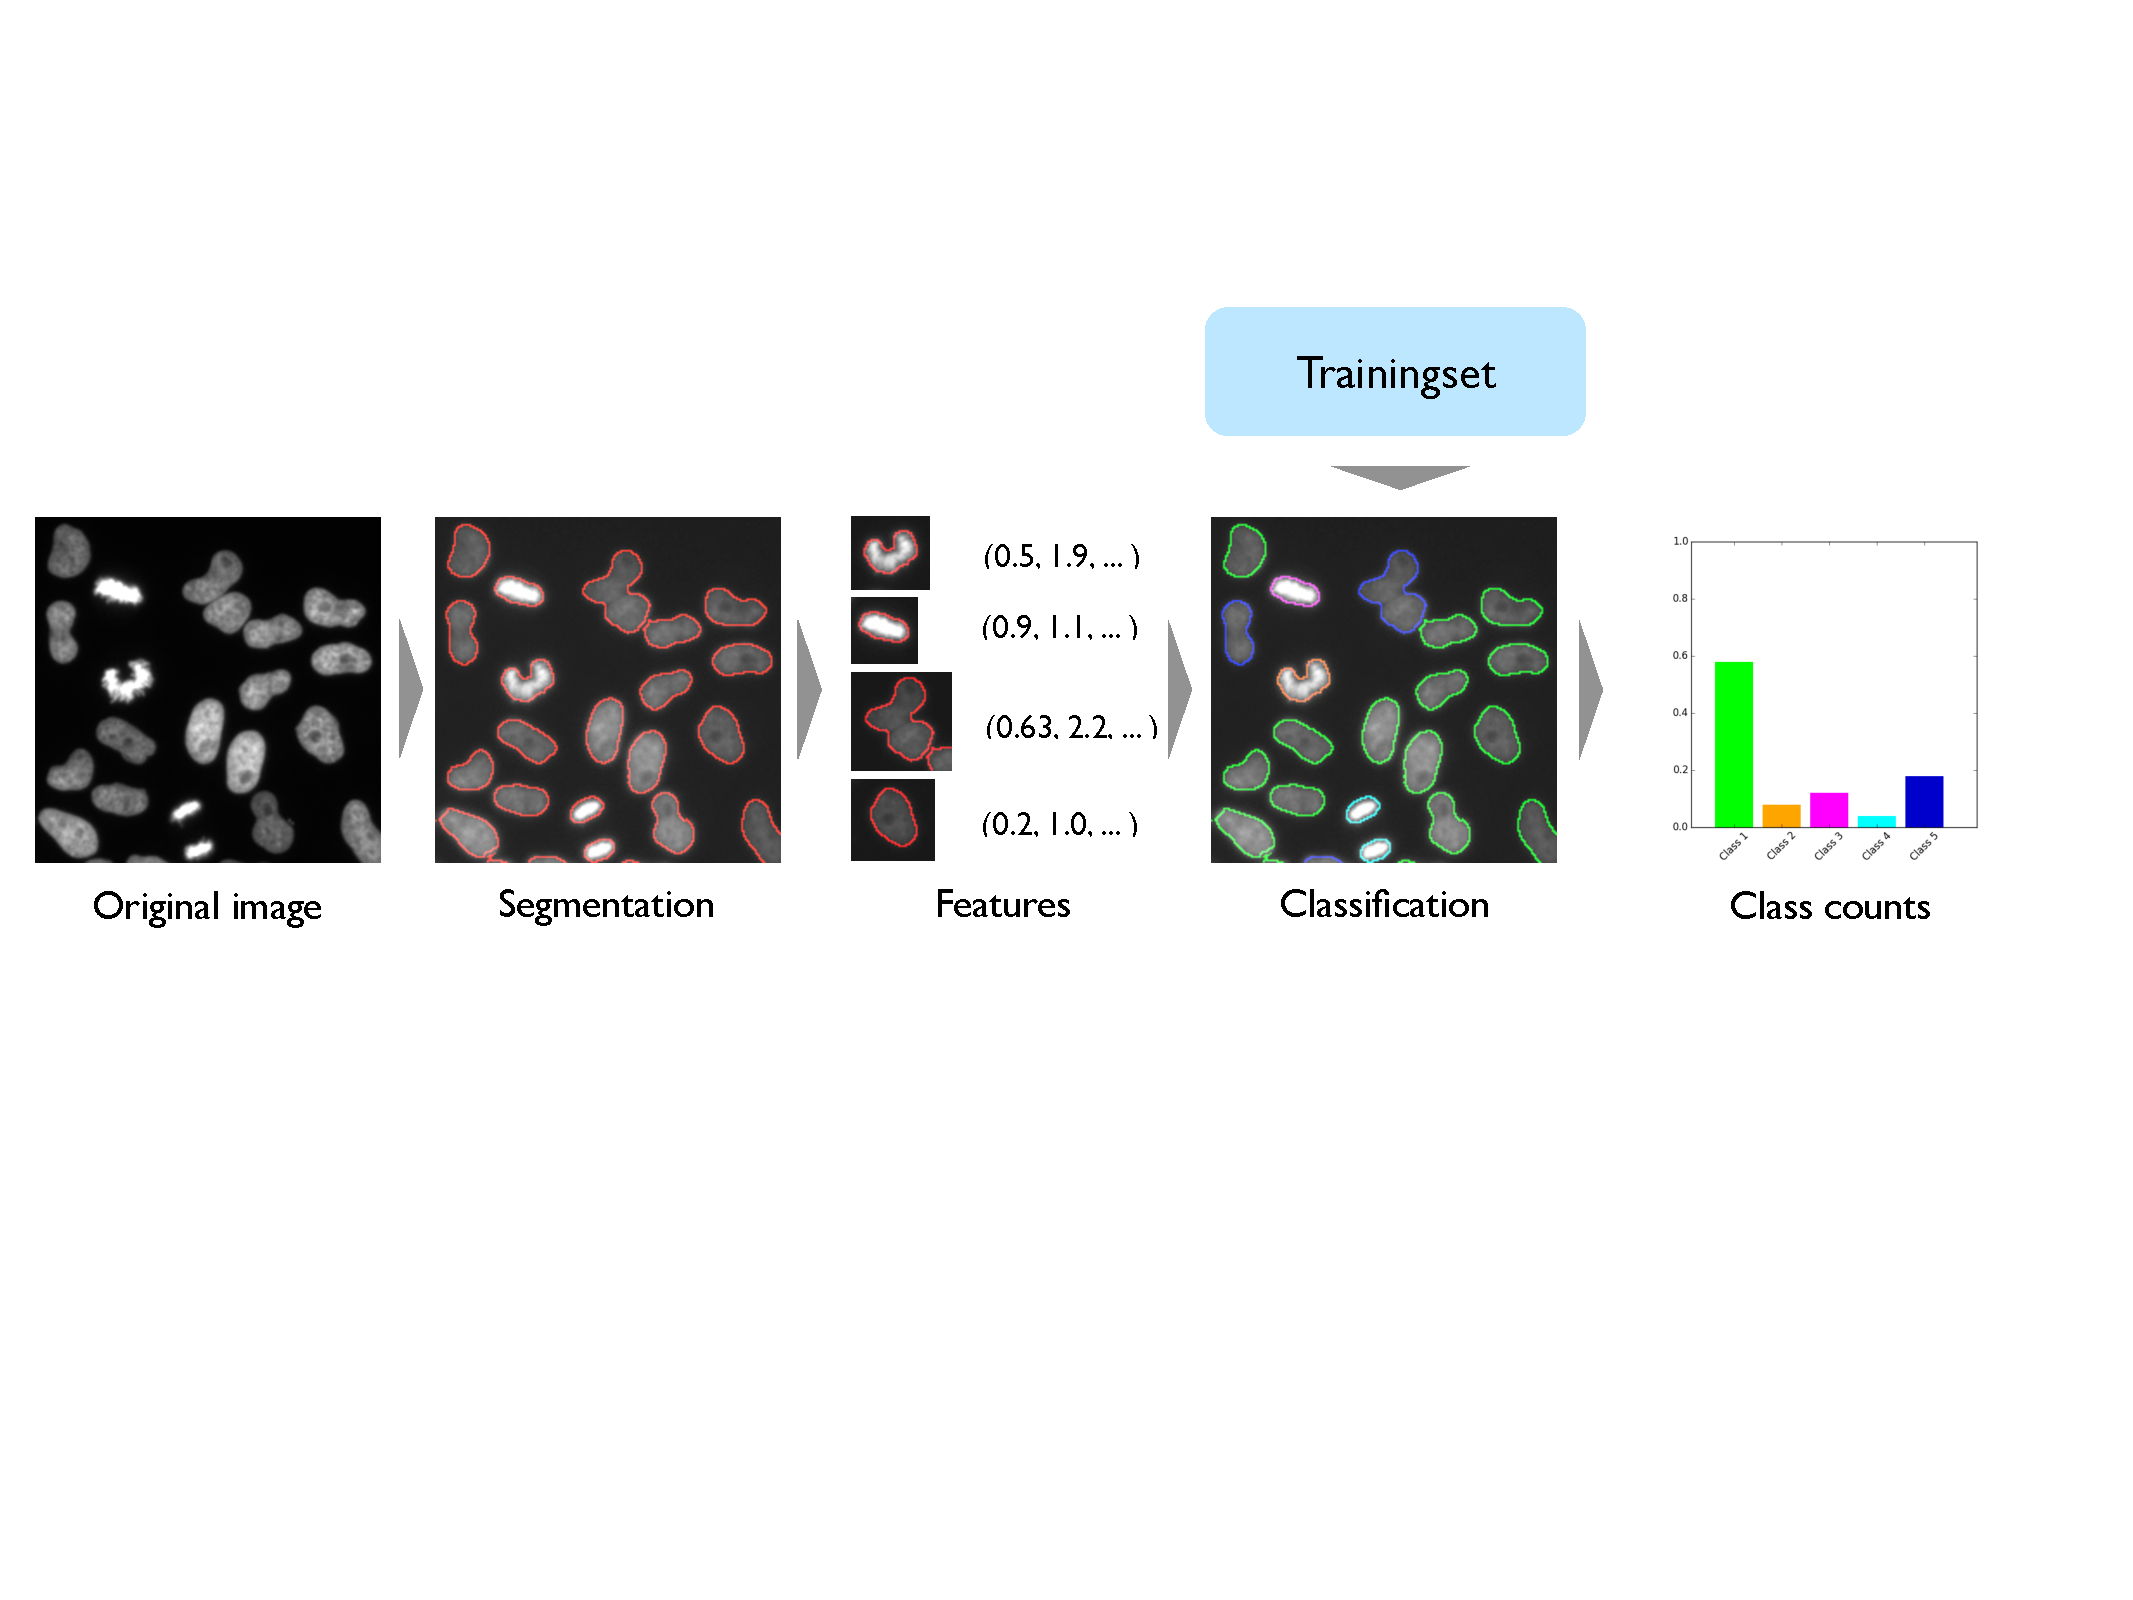
\includegraphics[width=0.8\textwidth]{../graphics/ComputationalPhenotyping.pdf}
% \end{figure}

% \begin{itemize}
% 	\item In this example, we wish to classify cell images. 
% 	\item For this, cells are first segmented and then described by a vector $x$ of features describing shape and texture. 
% 	\item We are given a training set $T = \{(x_i, y_i)\}_{i=1, \ldots, \nsize}$, i.e. for each cell in the training set, we know its morphological class. 
% 	\item The task is to infer a function $f$ from the training set that allows to assign one of these classes to new unseen objects.
% \end{itemize}
% \end{frame}

\begin{frame}{Example: classification of cells}
\begin{figure}[htb]
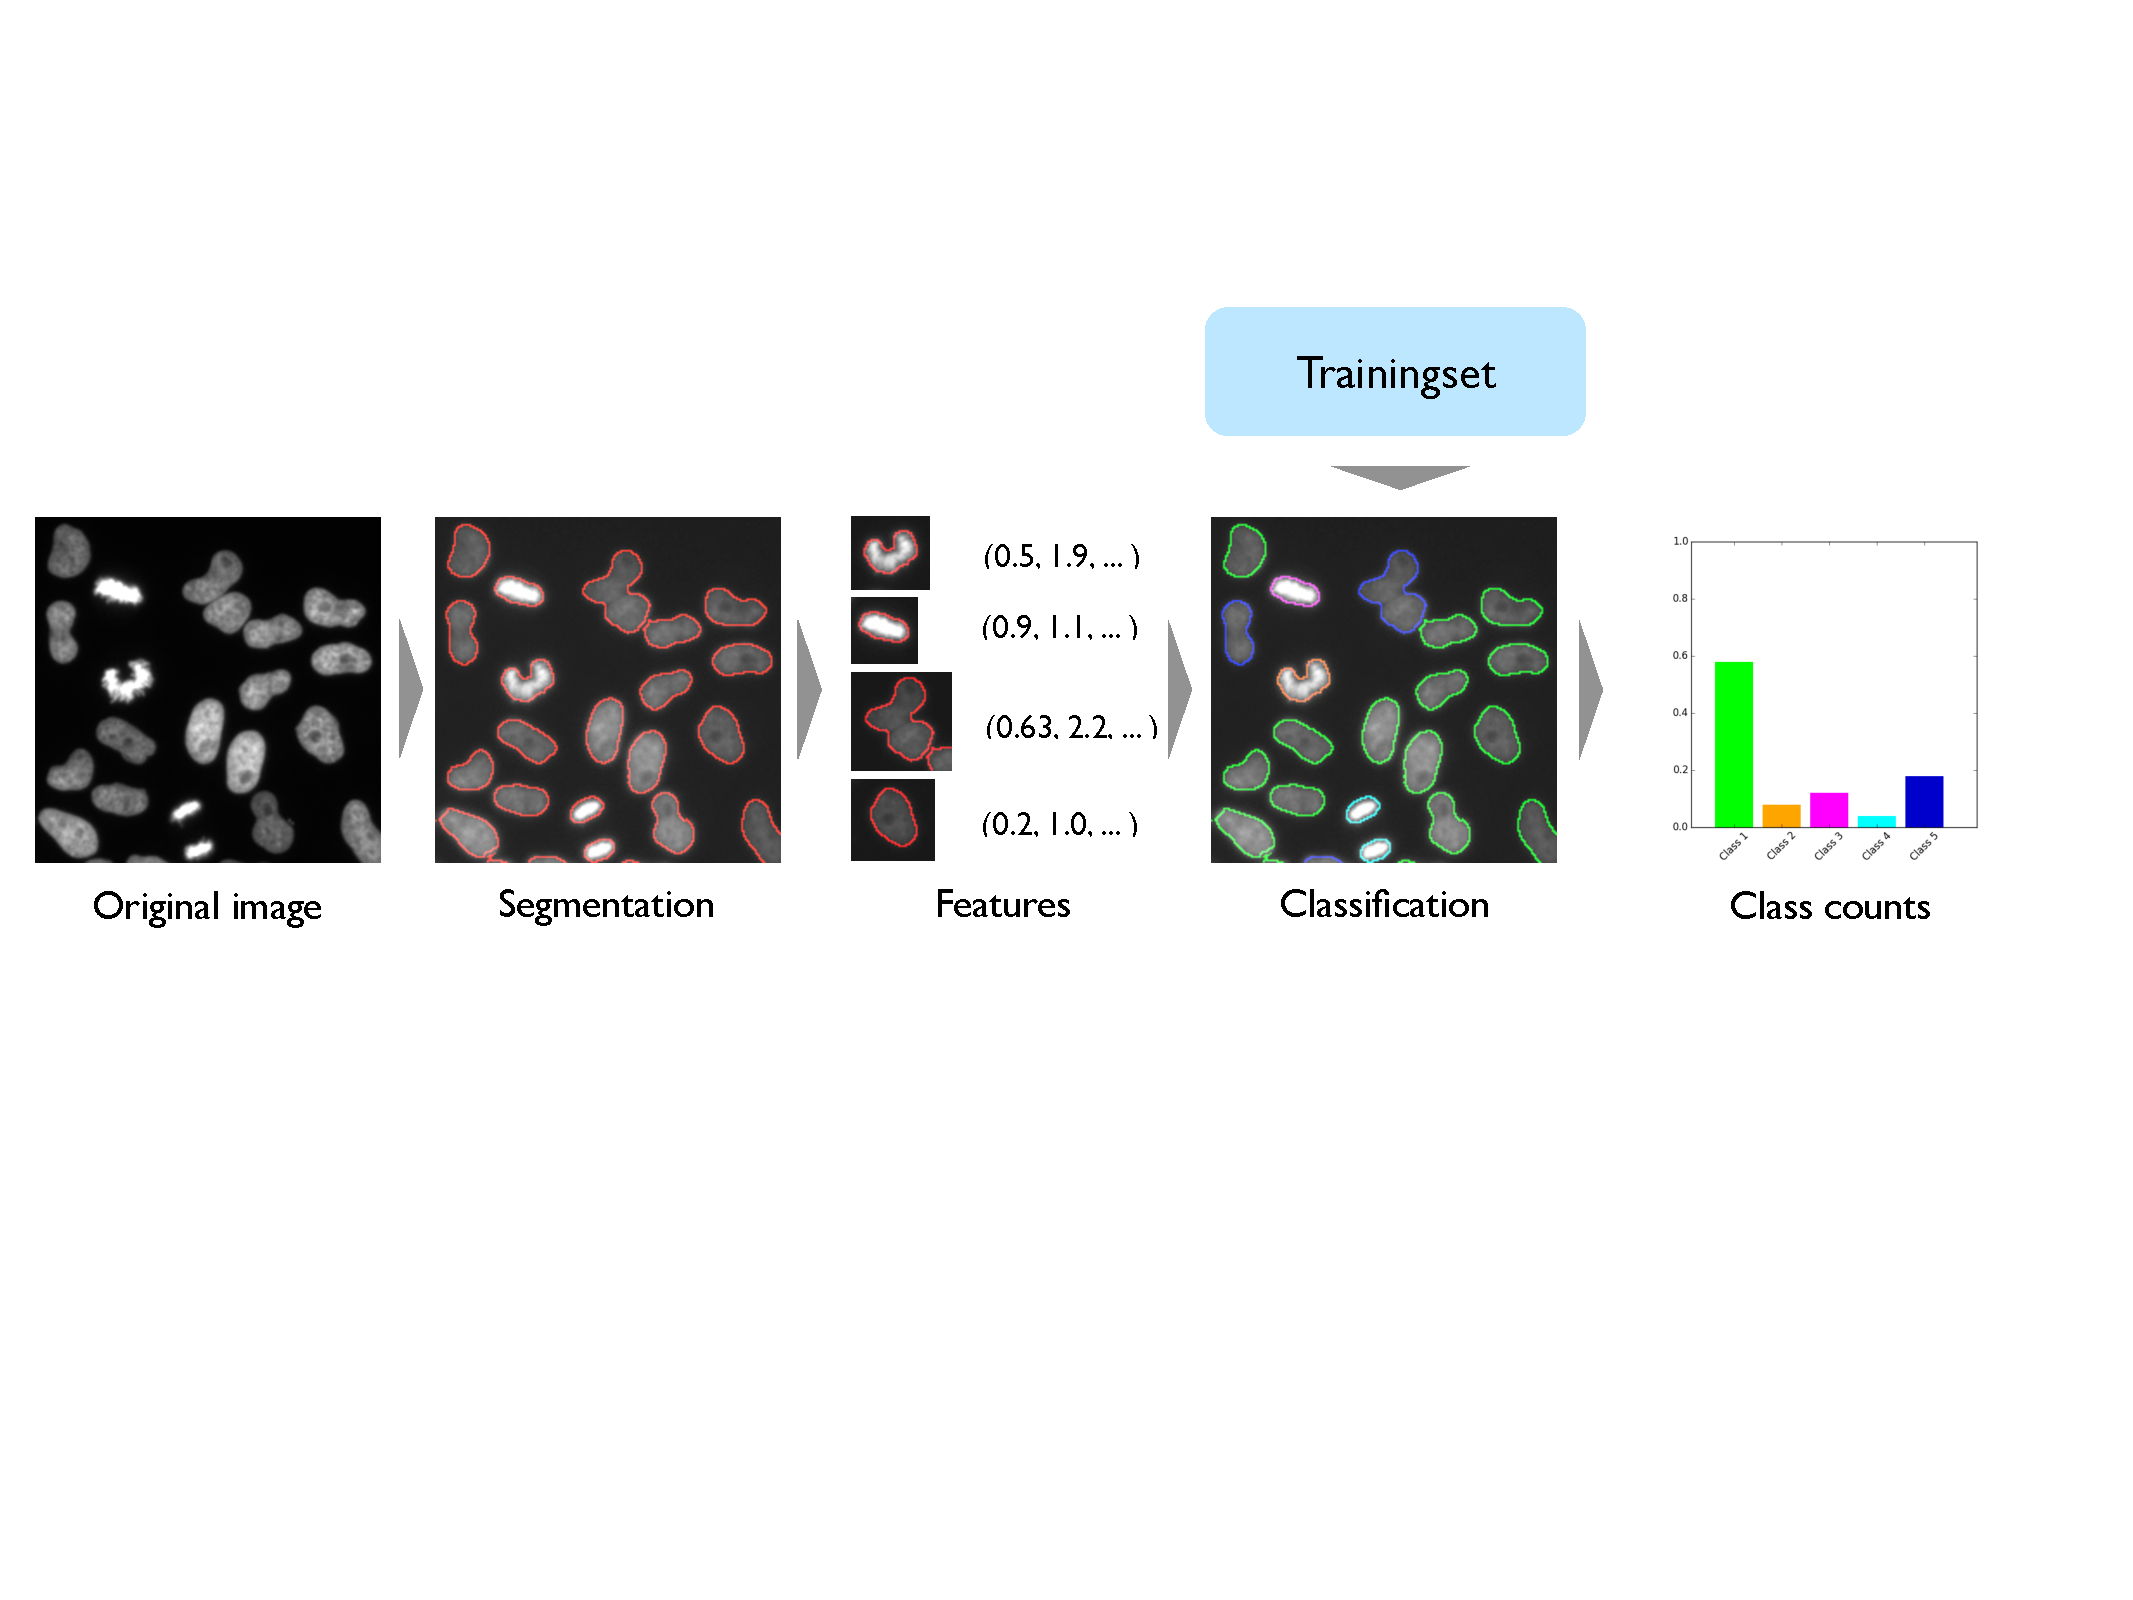
\includegraphics[width=0.8\textwidth]{../graphics/ComputationalPhenotyping.pdf}
\end{figure}

\begin{itemize}
	\item In this example, we wish to classify cell images. 
	\item For this, cells are first segmented and then represented by a vector $x \in \mathbb{R}^P$ of features describing shape and texture for each segmented object.
	%\item We define a set of morphological, biologically meaningful classes. 
	\item We are given a training set $T = \{(x_i, y_i)\}_{i=1, \ldots, \nsize}$, i.e. for each cell in the training set $x_i \in \mathbb{R}^P$, we know its morphological class $y_i$. 
	\item The task is to infer a function $f$ from the training set that allows to assign one of these classes to new unseen objects.
\end{itemize}
\end{frame}

%\subsection{Nearest Neighbor classification}
\subsection{Random Forests}

\begin{frame}{Random Forest: Decision trees}
\begin{figure}[htb]
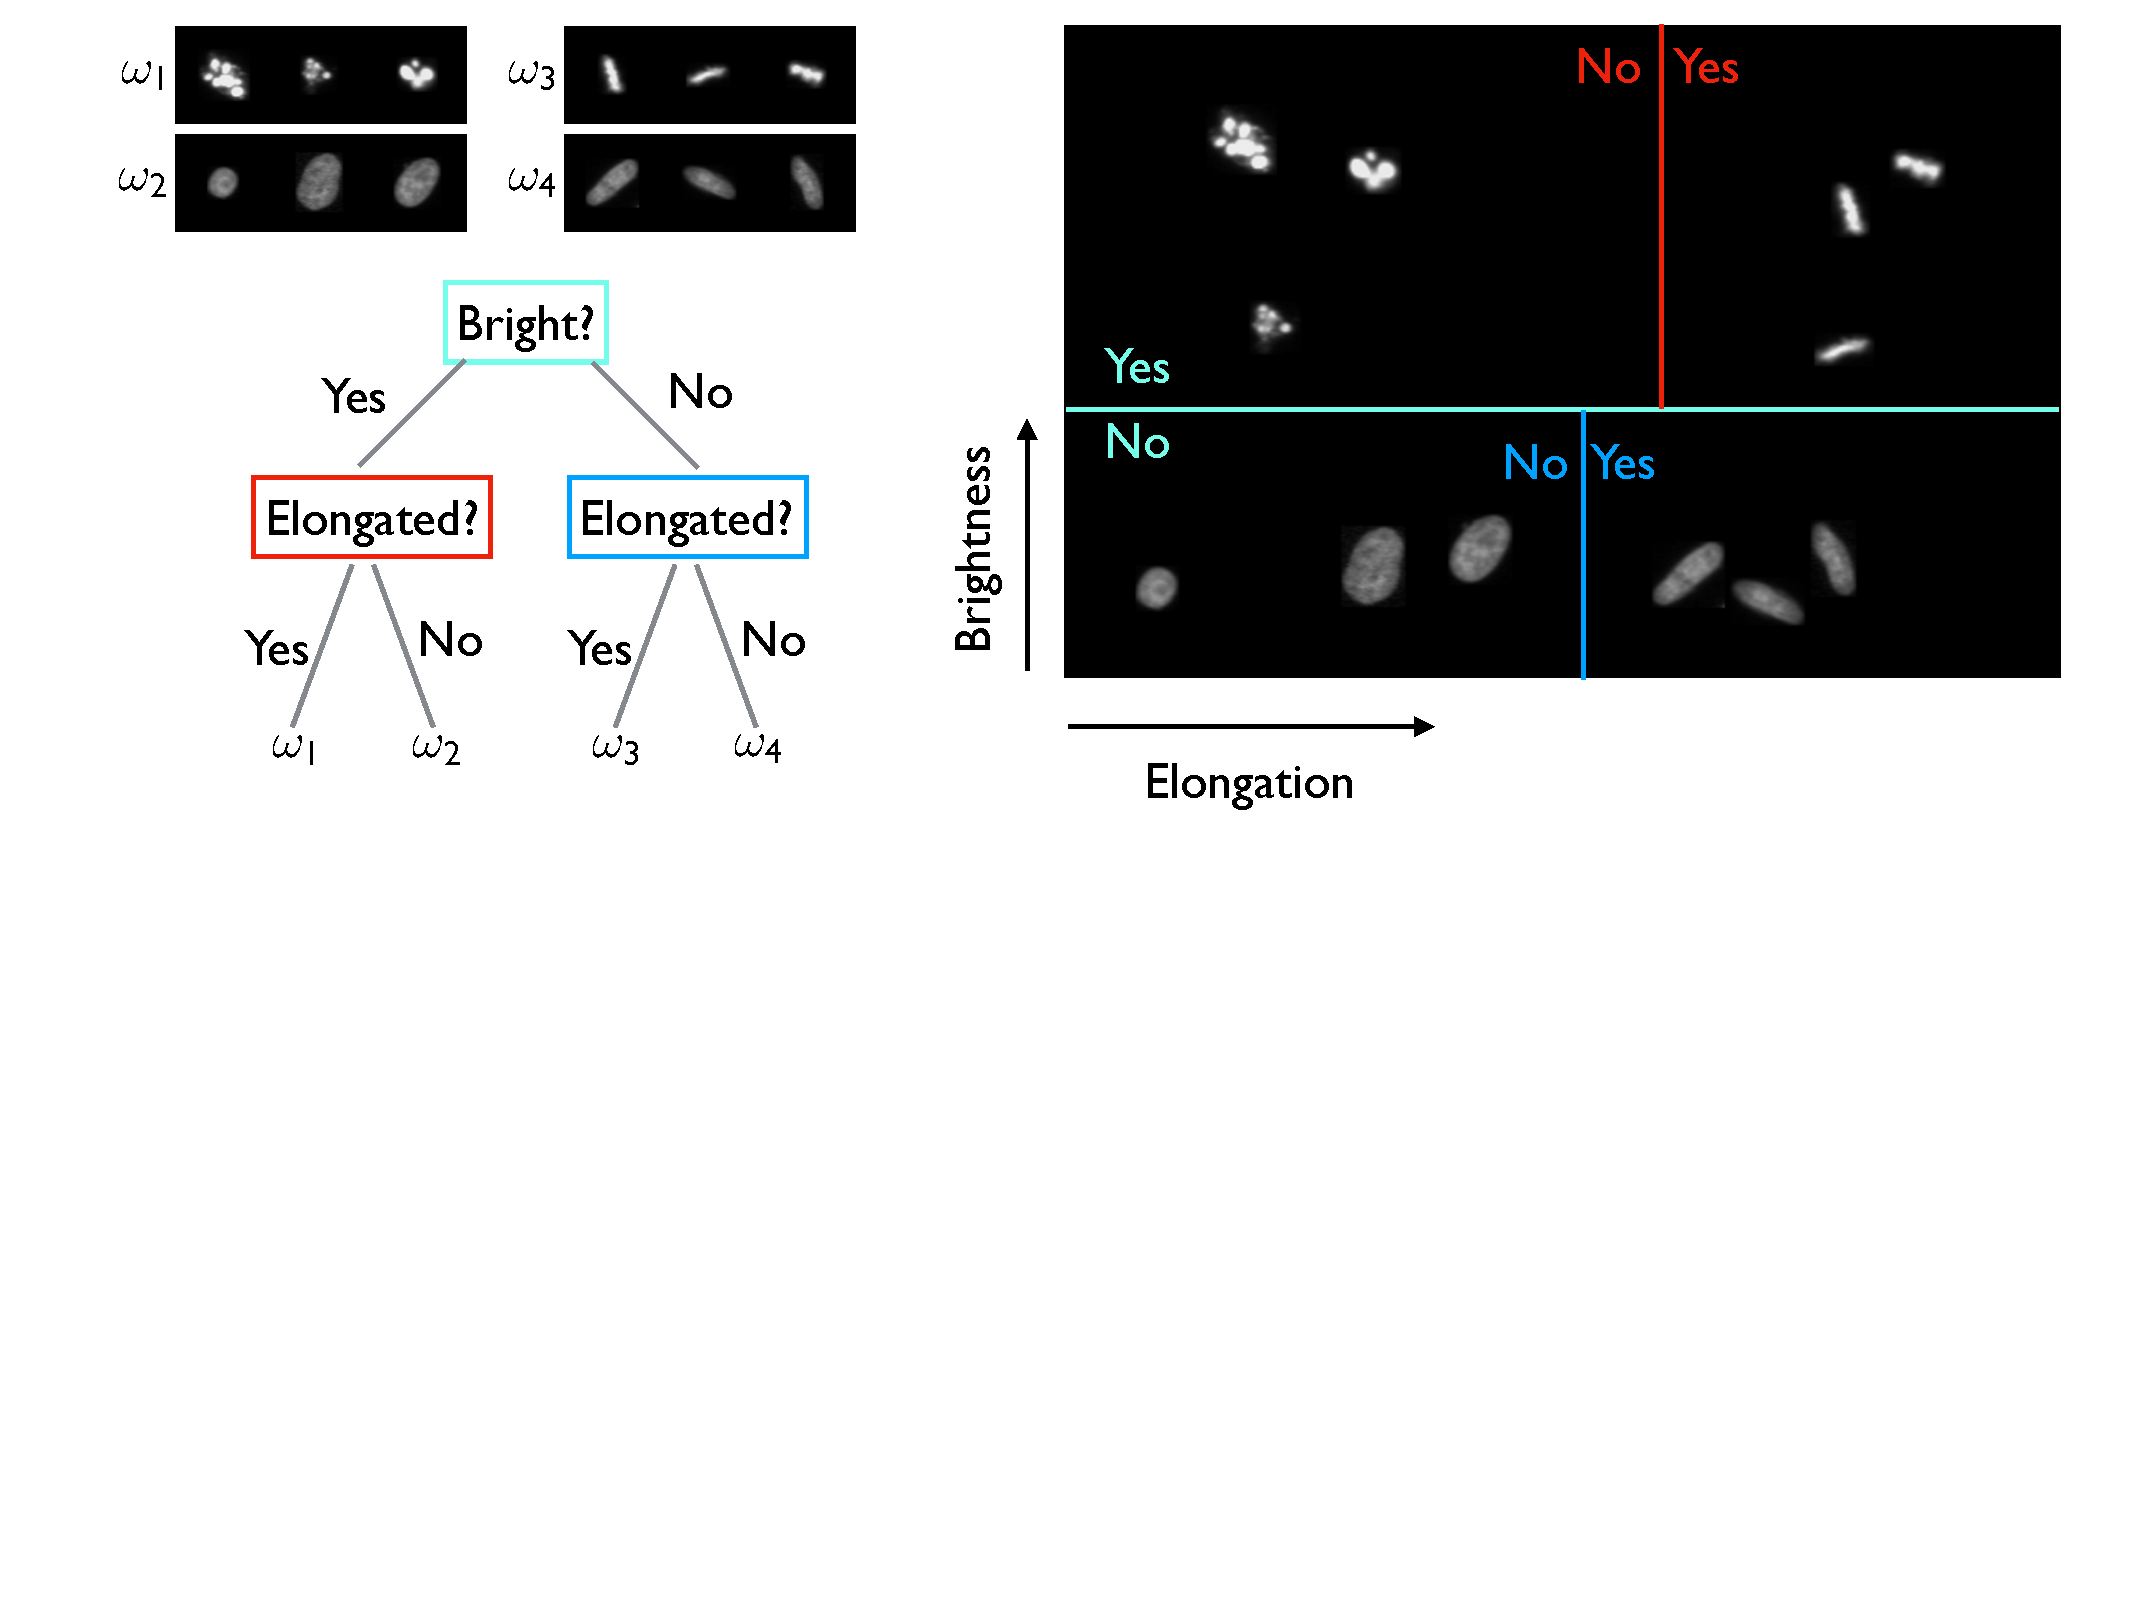
\includegraphics[width=0.8\textwidth]{../graphics/CellClassification_RF.pdf}
\end{figure}

\begin{itemize}
	\item Intuitive approach: applying a series of "rules" to the training data to recover the classes $\omega_i$ (e.g. "is the cell bright?", "is the cell elongated?", ... ) 	
	\item Each rule (or decision) divides the set of objects into two subsets. 
	\item The whole classifier is thus represented by a decision tree, i.e. a hierarchically organized set of binary decisions.
\end{itemize}
	
\end{frame}

\begin{frame}{Random Forest: Decision trees}
\begin{figure}[htb]
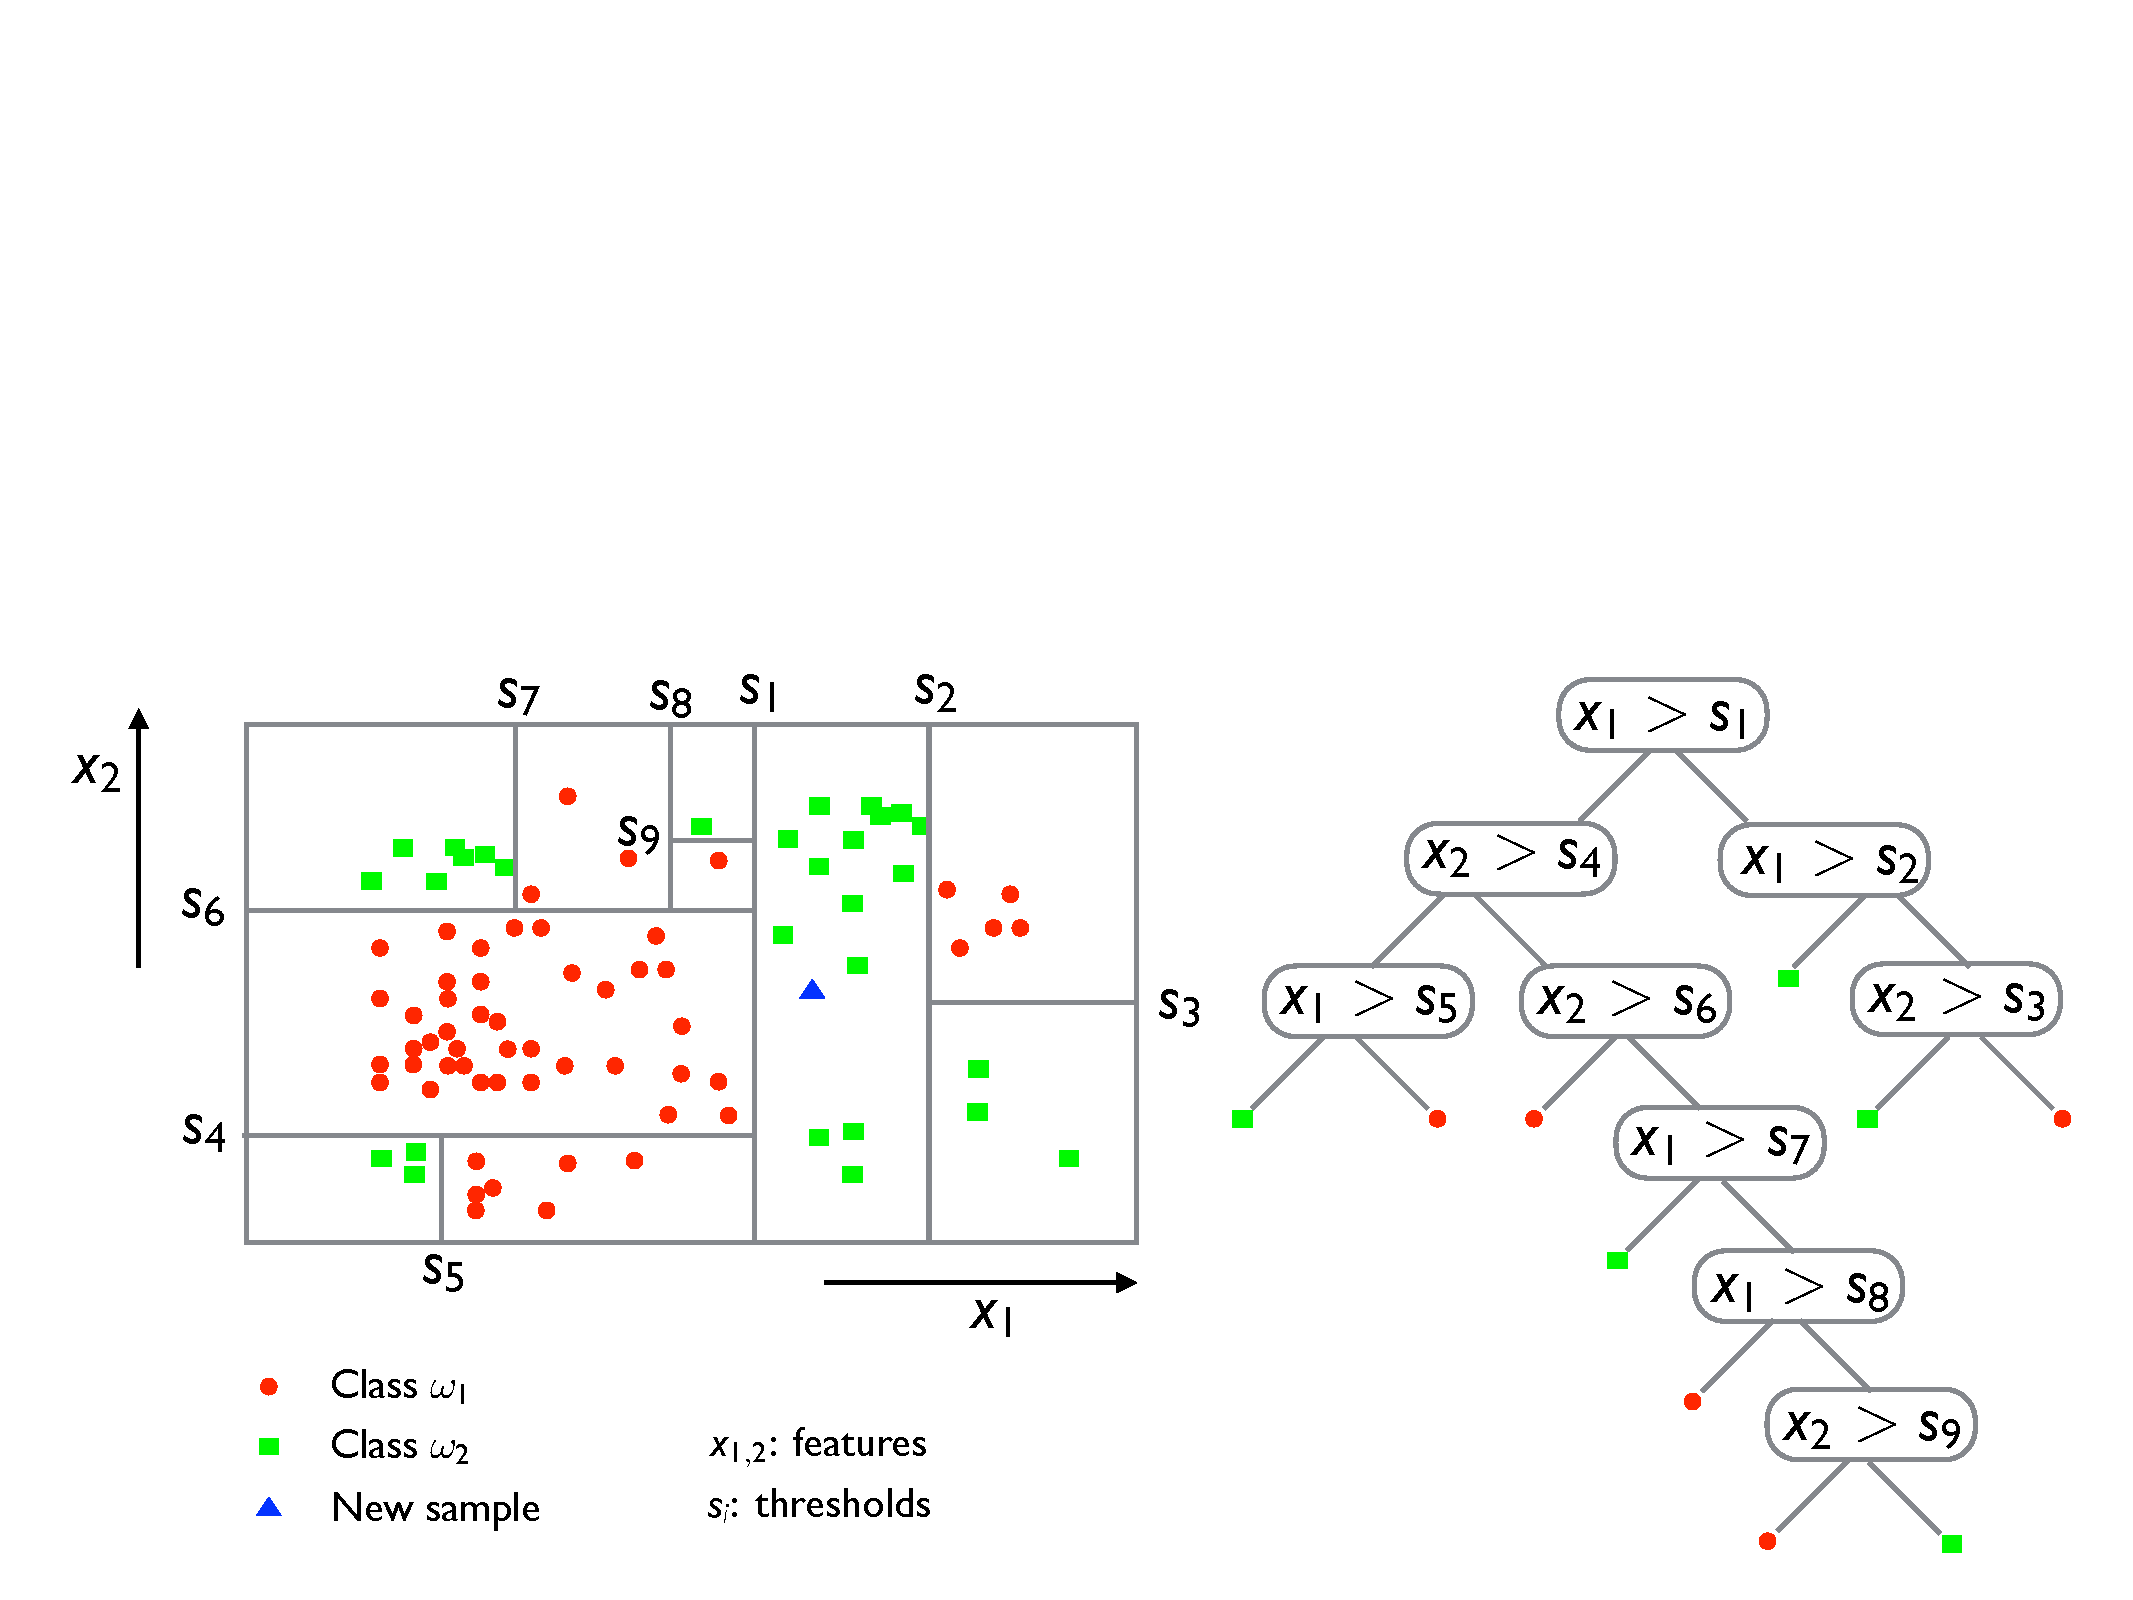
\includegraphics[width=0.8\textwidth]{../graphics/RF2.pdf}
\end{figure}

\begin{itemize}
	\item The decision tree corresponds to a partition of the feature space. 
	\item The corresponding decision boundaries can be very complex and adapts to the training set.
	\item Classification of a new object: application of the binary decision rules and assignment of the leaf label.
\end{itemize}
	
\end{frame}

\begin{frame}{Random Forest: Decision trees}
\begin{itemize}
\item Such decision trees can be built from data in an optimal way, by repeated division of the feature space. 
\item At every step, we split the data set into two, according to one feature. 
\item The feature and the threshold are chosen automatically in such a way that the resulting groups have best "purity".
\item This can be achieved by minimizing the GINI impurity. For $K$ classes, GINI impurity is defined as:
\begin{eqnarray*}
GI(R_m) &=& \sum_{k=1}^{K}\hat{p}_{mk}(1-\hat{p}_{mk}) \\
GI(s) &=& \sum_{R_m}=\frac{|R_m|}{N}GI(R_m)
\end{eqnarray*}
where $R_m$ are the sets resulting from the split $s$ and $\hat{p}_{mk}$ is the probability of a sample in $R_m$ to belong to class $k$.
\end{itemize}
\end{frame}


\subsection{Linear Discriminant Analysis (LDA)}
\subsection{Support Vector Machines (SVM) and kernel methods}

\section{Conclusion}


%%%%%%%%%%%%%%%%%%%%%%%%%%%%%%%%%%%%%%%%%%%%%%%%%%%%%%%%%%%%%%%%%%%%%%%%%
%%%%%%%%%%%%%%%%%%%%%%%%%%%%%%%%%%%%%%%%%%%%%%%%%%%%%%%%%%%%%%%%%%%%%%%%%
\section{References}
\begin{frame}[allowframebreaks]
	\frametitle{References}
	\bibliography{slides_deep.bib}
\end{frame}


\end{document}